\documentclass[]{article}
\usepackage{lmodern}
\usepackage{amssymb,amsmath}
\usepackage{ifxetex,ifluatex}
\usepackage{fixltx2e} % provides \textsubscript
\ifnum 0\ifxetex 1\fi\ifluatex 1\fi=0 % if pdftex
  \usepackage[T1]{fontenc}
  \usepackage[utf8]{inputenc}
\else % if luatex or xelatex
  \ifxetex
    \usepackage{mathspec}
  \else
    \usepackage{fontspec}
  \fi
  \defaultfontfeatures{Ligatures=TeX,Scale=MatchLowercase}
\fi
% use upquote if available, for straight quotes in verbatim environments
\IfFileExists{upquote.sty}{\usepackage{upquote}}{}
% use microtype if available
\IfFileExists{microtype.sty}{%
\usepackage{microtype}
\UseMicrotypeSet[protrusion]{basicmath} % disable protrusion for tt fonts
}{}
\usepackage[margin=1in]{geometry}
\usepackage{hyperref}
\hypersetup{unicode=true,
            pdftitle={Wauchier},
            pdfauthor={JB Camps},
            pdfborder={0 0 0},
            breaklinks=true}
\urlstyle{same}  % don't use monospace font for urls
\usepackage{color}
\usepackage{fancyvrb}
\newcommand{\VerbBar}{|}
\newcommand{\VERB}{\Verb[commandchars=\\\{\}]}
\DefineVerbatimEnvironment{Highlighting}{Verbatim}{commandchars=\\\{\}}
% Add ',fontsize=\small' for more characters per line
\usepackage{framed}
\definecolor{shadecolor}{RGB}{248,248,248}
\newenvironment{Shaded}{\begin{snugshade}}{\end{snugshade}}
\newcommand{\AlertTok}[1]{\textcolor[rgb]{0.94,0.16,0.16}{#1}}
\newcommand{\AnnotationTok}[1]{\textcolor[rgb]{0.56,0.35,0.01}{\textbf{\textit{#1}}}}
\newcommand{\AttributeTok}[1]{\textcolor[rgb]{0.77,0.63,0.00}{#1}}
\newcommand{\BaseNTok}[1]{\textcolor[rgb]{0.00,0.00,0.81}{#1}}
\newcommand{\BuiltInTok}[1]{#1}
\newcommand{\CharTok}[1]{\textcolor[rgb]{0.31,0.60,0.02}{#1}}
\newcommand{\CommentTok}[1]{\textcolor[rgb]{0.56,0.35,0.01}{\textit{#1}}}
\newcommand{\CommentVarTok}[1]{\textcolor[rgb]{0.56,0.35,0.01}{\textbf{\textit{#1}}}}
\newcommand{\ConstantTok}[1]{\textcolor[rgb]{0.00,0.00,0.00}{#1}}
\newcommand{\ControlFlowTok}[1]{\textcolor[rgb]{0.13,0.29,0.53}{\textbf{#1}}}
\newcommand{\DataTypeTok}[1]{\textcolor[rgb]{0.13,0.29,0.53}{#1}}
\newcommand{\DecValTok}[1]{\textcolor[rgb]{0.00,0.00,0.81}{#1}}
\newcommand{\DocumentationTok}[1]{\textcolor[rgb]{0.56,0.35,0.01}{\textbf{\textit{#1}}}}
\newcommand{\ErrorTok}[1]{\textcolor[rgb]{0.64,0.00,0.00}{\textbf{#1}}}
\newcommand{\ExtensionTok}[1]{#1}
\newcommand{\FloatTok}[1]{\textcolor[rgb]{0.00,0.00,0.81}{#1}}
\newcommand{\FunctionTok}[1]{\textcolor[rgb]{0.00,0.00,0.00}{#1}}
\newcommand{\ImportTok}[1]{#1}
\newcommand{\InformationTok}[1]{\textcolor[rgb]{0.56,0.35,0.01}{\textbf{\textit{#1}}}}
\newcommand{\KeywordTok}[1]{\textcolor[rgb]{0.13,0.29,0.53}{\textbf{#1}}}
\newcommand{\NormalTok}[1]{#1}
\newcommand{\OperatorTok}[1]{\textcolor[rgb]{0.81,0.36,0.00}{\textbf{#1}}}
\newcommand{\OtherTok}[1]{\textcolor[rgb]{0.56,0.35,0.01}{#1}}
\newcommand{\PreprocessorTok}[1]{\textcolor[rgb]{0.56,0.35,0.01}{\textit{#1}}}
\newcommand{\RegionMarkerTok}[1]{#1}
\newcommand{\SpecialCharTok}[1]{\textcolor[rgb]{0.00,0.00,0.00}{#1}}
\newcommand{\SpecialStringTok}[1]{\textcolor[rgb]{0.31,0.60,0.02}{#1}}
\newcommand{\StringTok}[1]{\textcolor[rgb]{0.31,0.60,0.02}{#1}}
\newcommand{\VariableTok}[1]{\textcolor[rgb]{0.00,0.00,0.00}{#1}}
\newcommand{\VerbatimStringTok}[1]{\textcolor[rgb]{0.31,0.60,0.02}{#1}}
\newcommand{\WarningTok}[1]{\textcolor[rgb]{0.56,0.35,0.01}{\textbf{\textit{#1}}}}
\usepackage{graphicx,grffile}
\makeatletter
\def\maxwidth{\ifdim\Gin@nat@width>\linewidth\linewidth\else\Gin@nat@width\fi}
\def\maxheight{\ifdim\Gin@nat@height>\textheight\textheight\else\Gin@nat@height\fi}
\makeatother
% Scale images if necessary, so that they will not overflow the page
% margins by default, and it is still possible to overwrite the defaults
% using explicit options in \includegraphics[width, height, ...]{}
\setkeys{Gin}{width=\maxwidth,height=\maxheight,keepaspectratio}
\IfFileExists{parskip.sty}{%
\usepackage{parskip}
}{% else
\setlength{\parindent}{0pt}
\setlength{\parskip}{6pt plus 2pt minus 1pt}
}
\setlength{\emergencystretch}{3em}  % prevent overfull lines
\providecommand{\tightlist}{%
  \setlength{\itemsep}{0pt}\setlength{\parskip}{0pt}}
\setcounter{secnumdepth}{0}
% Redefines (sub)paragraphs to behave more like sections
\ifx\paragraph\undefined\else
\let\oldparagraph\paragraph
\renewcommand{\paragraph}[1]{\oldparagraph{#1}\mbox{}}
\fi
\ifx\subparagraph\undefined\else
\let\oldsubparagraph\subparagraph
\renewcommand{\subparagraph}[1]{\oldsubparagraph{#1}\mbox{}}
\fi

%%% Use protect on footnotes to avoid problems with footnotes in titles
\let\rmarkdownfootnote\footnote%
\def\footnote{\protect\rmarkdownfootnote}

%%% Change title format to be more compact
\usepackage{titling}

% Create subtitle command for use in maketitle
\providecommand{\subtitle}[1]{
  \posttitle{
    \begin{center}\large#1\end{center}
    }
}

\setlength{\droptitle}{-2em}

  \title{Wauchier}
    \pretitle{\vspace{\droptitle}\centering\huge}
  \posttitle{\par}
    \author{JB Camps}
    \preauthor{\centering\large\emph}
  \postauthor{\par}
      \predate{\centering\large\emph}
  \postdate{\par}
    \date{23 novembre 2018 / 30 juin 2019 (Paris, Rome, Turin, Eurostar, )}


\begin{document}
\maketitle

\hypertarget{preparations}{%
\section{Preparations}\label{preparations}}

\hypertarget{load-libraries-and-functions}{%
\subsection{Load libraries and
functions}\label{load-libraries-and-functions}}

\begin{Shaded}
\begin{Highlighting}[]
\KeywordTok{library}\NormalTok{(}\StringTok{"cluster"}\NormalTok{)}
\KeywordTok{library}\NormalTok{(}\StringTok{"dendextend"}\NormalTok{)}
\end{Highlighting}
\end{Shaded}

\begin{verbatim}
## 
## ---------------------
## Welcome to dendextend version 1.12.0
## Type citation('dendextend') for how to cite the package.
## 
## Type browseVignettes(package = 'dendextend') for the package vignette.
## The github page is: https://github.com/talgalili/dendextend/
## 
## Suggestions and bug-reports can be submitted at: https://github.com/talgalili/dendextend/issues
## Or contact: <tal.galili@gmail.com>
## 
##  To suppress this message use:  suppressPackageStartupMessages(library(dendextend))
## ---------------------
\end{verbatim}

\begin{verbatim}
## 
## Attaching package: 'dendextend'
\end{verbatim}

\begin{verbatim}
## The following object is masked from 'package:stats':
## 
##     cutree
\end{verbatim}

\begin{Shaded}
\begin{Highlighting}[]
\KeywordTok{source}\NormalTok{(}\StringTok{"functions.R"}\NormalTok{)}
\end{Highlighting}
\end{Shaded}

\begin{verbatim}
## Loading required package: ggplot2
\end{verbatim}

\hypertarget{corpus-description-and-selection}{%
\section{Corpus description and
selection}\label{corpus-description-and-selection}}

\hypertarget{load-data}{%
\subsection{Load data}\label{load-data}}

\begin{Shaded}
\begin{Highlighting}[]
\CommentTok{# Get data with Stylo}
\CommentTok{# data = stylo::load.corpus.and.parse(corpus.dir = "~/dev/dh-meier/output/transkribus-etudiants/tokenized/boudams", features = "w", ngram.size = 1, preserve.case = FALSE)}
\CommentTok{# Get freq lists}
\CommentTok{#data = stylo::make.table.of.frequencies(corpus = data, features = unique(sort(unlist(data))), relative = FALSE)}
\CommentTok{# Write it}
\CommentTok{#write.csv(as.matrix(data), "data/transkr_student_expanded_words.csv")}
\NormalTok{data =}\StringTok{ }\KeywordTok{read.csv}\NormalTok{(}\StringTok{"data/transkr_student_expanded_words.csv"}\NormalTok{, }\DataTypeTok{header =} \OtherTok{TRUE}\NormalTok{, }\DataTypeTok{row.names =} \DecValTok{1}\NormalTok{)}
\NormalTok{data =}\StringTok{ }\KeywordTok{t}\NormalTok{(data)}
\end{Highlighting}
\end{Shaded}

\hypertarget{text-lengths}{%
\subsection{Text lengths}\label{text-lengths}}

\begin{Shaded}
\begin{Highlighting}[]
\NormalTok{nwords =}\StringTok{ }\KeywordTok{colSums}\NormalTok{(data)}
\KeywordTok{summary}\NormalTok{(nwords)}
\end{Highlighting}
\end{Shaded}

\begin{verbatim}
##    Min. 1st Qu.  Median    Mean 3rd Qu.    Max. 
##       7    2288    3420    5002    6740   18979
\end{verbatim}

\begin{Shaded}
\begin{Highlighting}[]
\KeywordTok{boxplot}\NormalTok{(nwords)}
\KeywordTok{boxplot}\NormalTok{(nwords)}\OperatorTok{$}\NormalTok{out}
\end{Highlighting}
\end{Shaded}

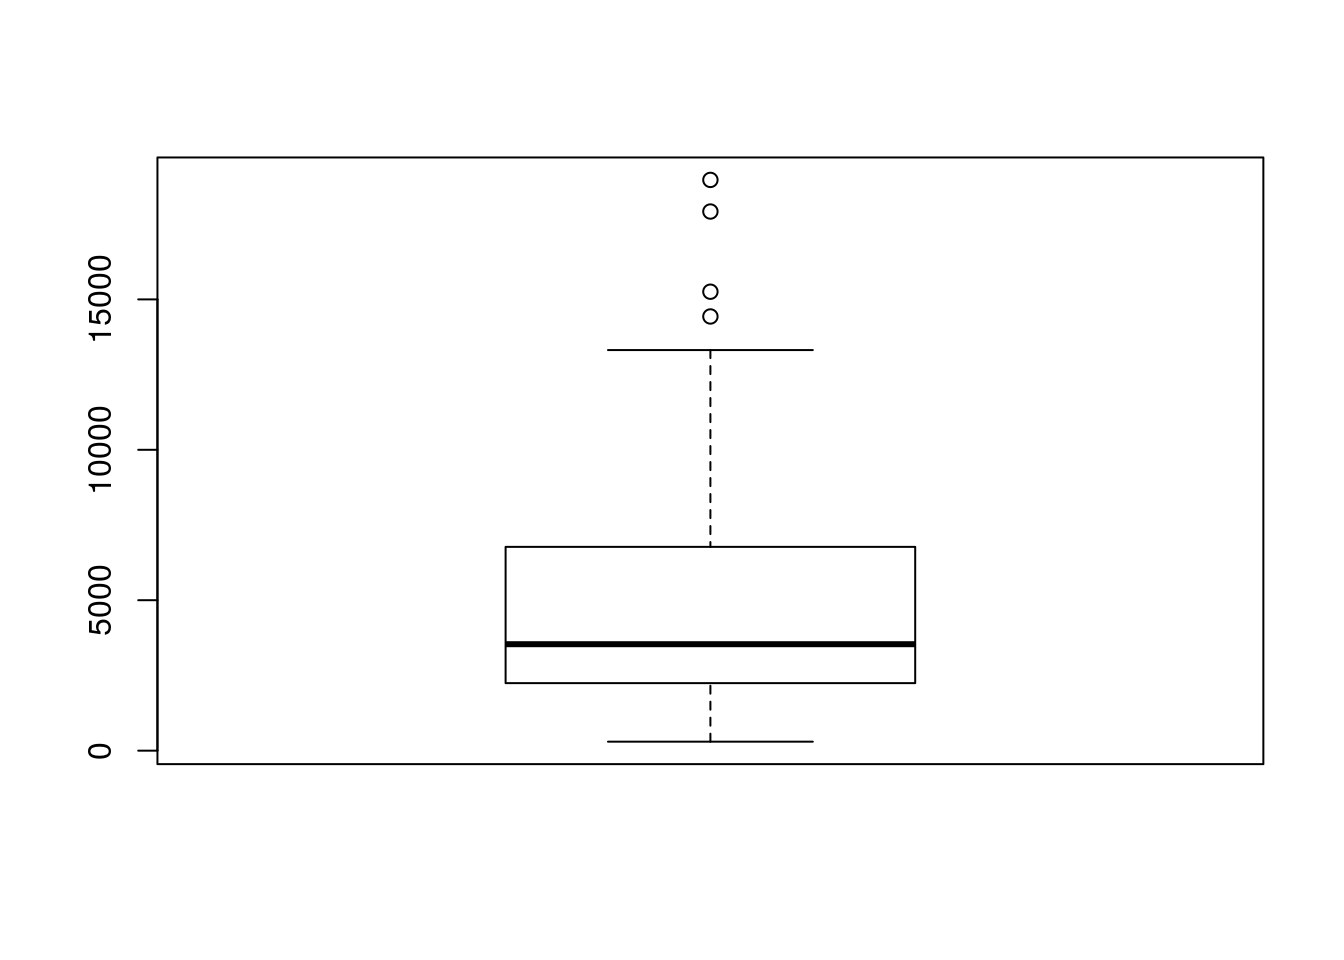
\includegraphics{Wauchier-Students_files/figure-latex/unnamed-chunk-3-1.pdf}

\begin{verbatim}
##         05_y_Leg-_A_Ap__tr_Vie  29_Wau_Leg-C_Co_Ev_Vie_Martin 
##                          17924                          14432 
## 31_Wau_Leg-C_Co_Ev_Dia_Martin3 34_Wau_Leg-C_Co_Ev_Vie_Martial 
##                          18979                          15262
\end{verbatim}

\begin{Shaded}
\begin{Highlighting}[]
\KeywordTok{head}\NormalTok{(}\KeywordTok{sort}\NormalTok{(nwords), }\DataTypeTok{n =} \DecValTok{15}\NormalTok{)}
\end{Highlighting}
\end{Shaded}

\begin{verbatim}
##            60_Ano_Leg-B_NA_NA_NA_Antechriste 
##                                            7 
## Item_Aut_Leg-Légendier_Cl_so__TitreRaccourci 
##                                            7 
##                  03_Ano_Leg-A_Ap_NA_Mar_Jean 
##                                          290 
##                  62_Ano_Leg-N_NA_NA_NA_Index 
##                                          327 
##               61_Ano_Leg-B_NA_NA_NA_Jugement 
##                                          384 
##               30_Wau_Leg-C_Co_Ev_Tra_Martin2 
##                                          722 
##              08_Ano_Leg-A_Ap_NA_Vie_Philippe 
##                                         1017 
##                 32_Wau_Leg-C_Co_Ev_Vie_Brice 
##                                         1376 
##         09_Ano_Leg-A_Ap_NA_Vie_JacquesMineur 
##                                         1379 
##               54_Ano_Leg-C_Vi_NA_Vie_Pelagie 
##                                         1500 
##              20_Ano_Leg-B_Ma_Fe_Vie_Felicite 
##                                         1685 
##                  11_Ano_Leg-A_Ap_NA_Vie_Marc 
##                                         1820 
##                 23_Ano_Leg-B_Ma_Ho_Vie_Sixte 
##                                         1900 
##            53_Ano_Leg-C_Vi_NA_Vie_Marguerite 
##                                         1941 
##               35_Wau_Leg-C_Co_Ev_Vie_Nicolas 
##                                         1954
\end{verbatim}

\begin{Shaded}
\begin{Highlighting}[]
\NormalTok{toKeep =}\StringTok{ }\KeywordTok{colnames}\NormalTok{(data)[nwords }\OperatorTok{>}\StringTok{ }\DecValTok{1000}\NormalTok{]}

\NormalTok{toKeep =}\StringTok{ }\NormalTok{toKeep[}\KeywordTok{grep}\NormalTok{(}\StringTok{"Bestiaire"}\NormalTok{, toKeep, }\DataTypeTok{invert =} \OtherTok{TRUE}\NormalTok{)]}

\NormalTok{df =}\StringTok{ }\KeywordTok{as.data.frame}\NormalTok{(nwords)}

\KeywordTok{ggplot}\NormalTok{(df, }\KeywordTok{aes}\NormalTok{(}\DataTypeTok{x=}\StringTok{""}\NormalTok{, }\DataTypeTok{y=}\NormalTok{nwords)) }\OperatorTok{+}\StringTok{ }\KeywordTok{geom_violin}\NormalTok{() }\OperatorTok{+}\StringTok{ }\KeywordTok{geom_boxplot}\NormalTok{(}\DataTypeTok{width=}\FloatTok{0.3}\NormalTok{) }\OperatorTok{+}\StringTok{  }\KeywordTok{theme}\NormalTok{(}\DataTypeTok{axis.text.y =} \KeywordTok{element_text}\NormalTok{(}\DataTypeTok{size =} \KeywordTok{rel}\NormalTok{(}\FloatTok{1.4}\NormalTok{)), }\DataTypeTok{axis.title =} \KeywordTok{element_text}\NormalTok{(}\DataTypeTok{size =} \KeywordTok{rel}\NormalTok{(}\FloatTok{1.4}\NormalTok{))) }\OperatorTok{+}\StringTok{ }\KeywordTok{xlab}\NormalTok{(}\StringTok{"Est. length in words of corpus texts"}\NormalTok{) }\OperatorTok{+}\StringTok{ }\KeywordTok{scale_y_continuous}\NormalTok{(}\DataTypeTok{breaks=}\KeywordTok{c}\NormalTok{(}\DecValTok{0}\NormalTok{, }\DecValTok{2500}\NormalTok{, }\DecValTok{5000}\NormalTok{, }\DecValTok{7500}\NormalTok{, }\DecValTok{10000}\NormalTok{, }\DecValTok{12500}\NormalTok{, }\DecValTok{15000}\NormalTok{, }\DecValTok{17500}\NormalTok{))}
\end{Highlighting}
\end{Shaded}

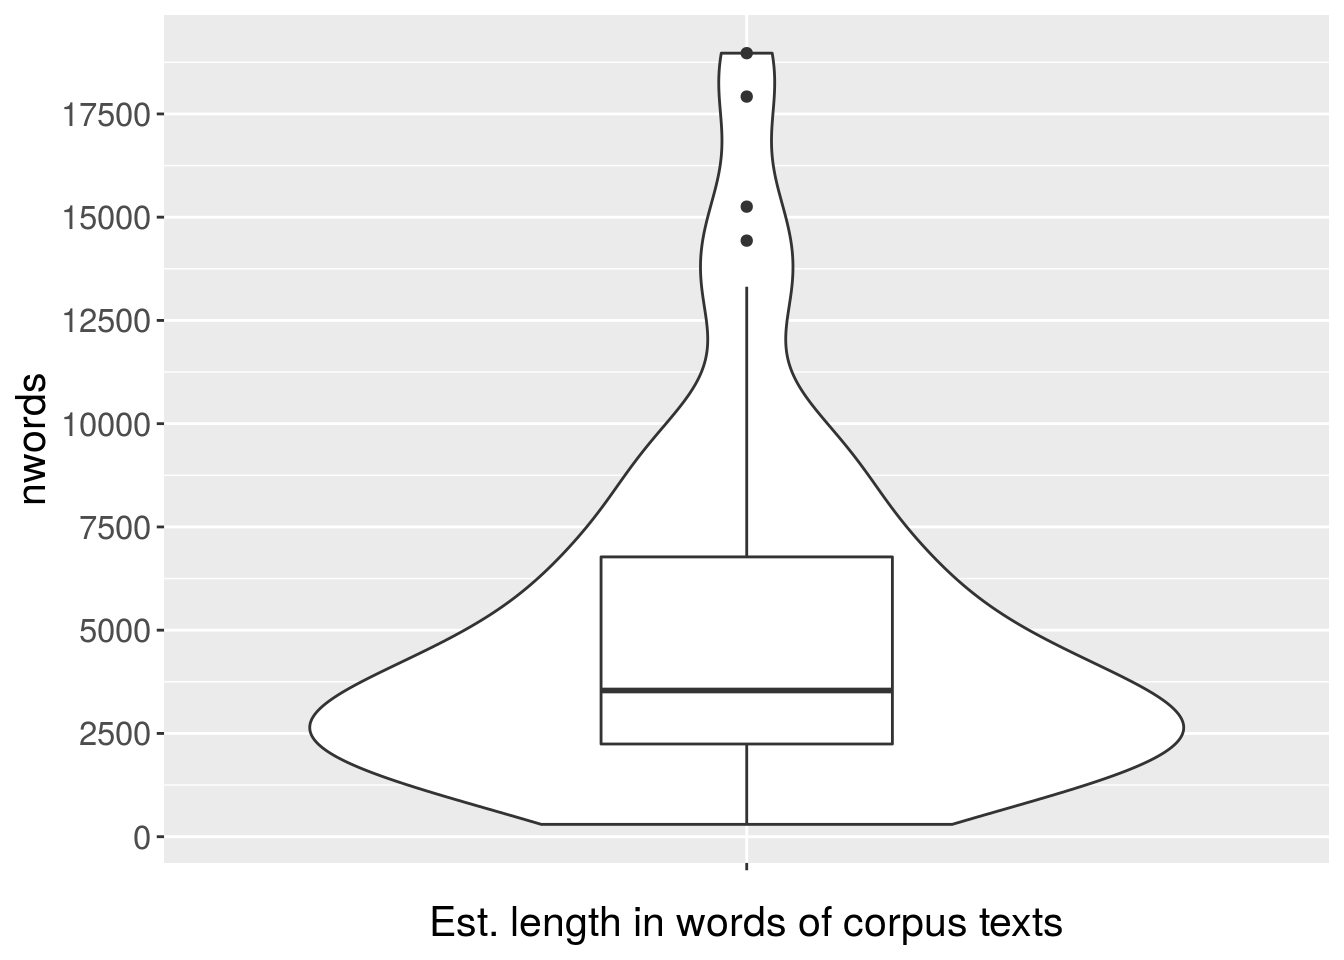
\includegraphics{Wauchier-Students_files/figure-latex/unnamed-chunk-3-2.pdf}

\hypertarget{transkribus-raw-data}{%
\section{Transkribus raw data}\label{transkribus-raw-data}}

\hypertarget{grams-from-raw-data}{%
\subsection{3-grams from raw data}\label{grams-from-raw-data}}

\hypertarget{load-data-1}{%
\subsection{Load data}\label{load-data-1}}

\begin{Shaded}
\begin{Highlighting}[]
\CommentTok{# Get data with Stylo}
\CommentTok{#data = stylo::load.corpus.and.parse(corpus.dir = "~/dev/dh-meier/output/transkribus-etudiants/raw/", features = "c", ngram.size = 3, preserve.case = FALSE)}
\CommentTok{# Get freq lists}
\CommentTok{#data = stylo::make.table.of.frequencies(corpus = data, features = unique(sort(unlist(data))), relative = FALSE)}
\CommentTok{# Write it}
\CommentTok{#write.csv(as.matrix(data), "data/transkr_student_raw_char3grams.csv")}
\NormalTok{data =}\StringTok{ }\KeywordTok{read.csv}\NormalTok{(}\StringTok{"data/transkr_student_raw_char3grams.csv"}\NormalTok{, }\DataTypeTok{header =} \OtherTok{TRUE}\NormalTok{, }\DataTypeTok{row.names =} \DecValTok{1}\NormalTok{)}
\NormalTok{data =}\StringTok{ }\KeywordTok{t}\NormalTok{(data)}
\NormalTok{data =}\StringTok{ }\NormalTok{data[, toKeep]}
\NormalTok{data =}\StringTok{ }\NormalTok{data[}\KeywordTok{rowSums}\NormalTok{(data) }\OperatorTok{>}\StringTok{ }\DecValTok{0}\NormalTok{, ]}
\end{Highlighting}
\end{Shaded}

\hypertarget{burrows-vector-length-norm}{%
\subsubsection{Burrows + vector-length
norm}\label{burrows-vector-length-norm}}

\begin{Shaded}
\begin{Highlighting}[]
\NormalTok{d =}\StringTok{ }\NormalTok{data}
\CommentTok{# Selection based on Moisl 2011}
\NormalTok{select =}\StringTok{ }\KeywordTok{selection}\NormalTok{(d, }\DataTypeTok{z =} \FloatTok{1.645}\NormalTok{)}
\NormalTok{select =}\StringTok{ }\NormalTok{select[,}\DecValTok{4}\NormalTok{]}
\CommentTok{# Normalisations}
\NormalTok{d =}\StringTok{ }\KeywordTok{relativeFreqs}\NormalTok{(d)}
\CommentTok{# save data for robustness checks}
\NormalTok{Raw3grSave =}\StringTok{ }\NormalTok{d}
\NormalTok{d =}\StringTok{ }\NormalTok{d[select,]}
\NormalTok{d =}\StringTok{ }\KeywordTok{normalisations}\NormalTok{(d)}
\NormalTok{myCAH =}\StringTok{ }\NormalTok{cluster}\OperatorTok{::}\KeywordTok{agnes}\NormalTok{(}\KeywordTok{t}\NormalTok{(d), }\DataTypeTok{metric =} \StringTok{"manhattan"}\NormalTok{, }\DataTypeTok{method=}\StringTok{"ward"}\NormalTok{)}
\CommentTok{# Save}
\NormalTok{CAHRaw3gr =}\StringTok{ }\NormalTok{myCAH}
\CommentTok{#TODO: heights}
\CommentTok{# barplot(sort(myCAH$height))}
\NormalTok{plotRaw3grams =}\StringTok{ }\KeywordTok{cahPlotCol}\NormalTok{(myCAH, }\DataTypeTok{k =} \DecValTok{9}\NormalTok{, }\DataTypeTok{main =} \StringTok{"Characters 3-grams from raw data (Transkr)"}\NormalTok{)}

\NormalTok{somCAH =}\StringTok{ }\KeywordTok{somCluster}\NormalTok{(d)}
\NormalTok{somplotRaw3grams =}\StringTok{ }\KeywordTok{cahPlotCol}\NormalTok{(somCAH, }\DataTypeTok{k =} \DecValTok{9}\NormalTok{, }\DataTypeTok{main =} \StringTok{"SOM BASED - Characters 3-grams from raw data (Transkr)"}\NormalTok{)}
\end{Highlighting}
\end{Shaded}

\hypertarget{transkribus-expanded-data}{%
\section{Transkribus expanded data}\label{transkribus-expanded-data}}

\hypertarget{load-data-2}{%
\subsection{Load data}\label{load-data-2}}

\begin{Shaded}
\begin{Highlighting}[]
\NormalTok{data =}\StringTok{ }\KeywordTok{read.csv}\NormalTok{(}\StringTok{"data/transkr_student_expanded_words.csv"}\NormalTok{, }\DataTypeTok{header =} \OtherTok{TRUE}\NormalTok{, }\DataTypeTok{row.names =} \DecValTok{1}\NormalTok{)}
\NormalTok{data =}\StringTok{ }\KeywordTok{t}\NormalTok{(data)}
\NormalTok{data =}\StringTok{ }\NormalTok{data[, toKeep]}
\NormalTok{data =}\StringTok{ }\NormalTok{data[}\KeywordTok{rowSums}\NormalTok{(data) }\OperatorTok{>}\StringTok{ }\DecValTok{0}\NormalTok{, ]}
\end{Highlighting}
\end{Shaded}

\hypertarget{forms-from-expanded-data}{%
\subsection{Forms from expanded data}\label{forms-from-expanded-data}}

\hypertarget{burrows-vector-length-norm-1}{%
\subsubsection{Burrows + vector-length
norm}\label{burrows-vector-length-norm-1}}

\begin{Shaded}
\begin{Highlighting}[]
\NormalTok{d =}\StringTok{ }\NormalTok{data}
\CommentTok{# Selection based on Moisl 2011}
\NormalTok{select =}\StringTok{ }\KeywordTok{selection}\NormalTok{(d, }\DataTypeTok{z =} \FloatTok{1.645}\NormalTok{)}
\NormalTok{select =}\StringTok{ }\NormalTok{select[,}\DecValTok{4}\NormalTok{]}
\CommentTok{# Normalisations}
\NormalTok{d =}\StringTok{ }\KeywordTok{relativeFreqs}\NormalTok{(d)}
\CommentTok{# save data for robustness checks}
\NormalTok{WordsSave =}\StringTok{ }\NormalTok{d}
\NormalTok{d =}\StringTok{ }\NormalTok{d[select,]}
\NormalTok{d =}\StringTok{ }\KeywordTok{normalisations}\NormalTok{(d)}
\NormalTok{myCAH =}\StringTok{ }\NormalTok{cluster}\OperatorTok{::}\KeywordTok{agnes}\NormalTok{(}\KeywordTok{t}\NormalTok{(d), }\DataTypeTok{metric =} \StringTok{"manhattan"}\NormalTok{, }\DataTypeTok{method=}\StringTok{"ward"}\NormalTok{)}
\CommentTok{# Save}
\NormalTok{CAHForms =}\StringTok{ }\NormalTok{myCAH}
\CommentTok{#TODO: heights}
\CommentTok{# barplot(sort(myCAH$height))}
\NormalTok{plotForms =}\StringTok{ }\KeywordTok{cahPlotCol}\NormalTok{(myCAH, }\DataTypeTok{k =} \DecValTok{9}\NormalTok{, }\DataTypeTok{main =} \StringTok{"Expanded word forms (Transkr/Boudams/Pie)"}\NormalTok{)}

\NormalTok{somCAH =}\StringTok{ }\KeywordTok{somCluster}\NormalTok{(d)}
\NormalTok{somplotForms =}\StringTok{ }\KeywordTok{cahPlotCol}\NormalTok{(somCAH, }\DataTypeTok{k =} \DecValTok{9}\NormalTok{, }\DataTypeTok{main =} \StringTok{"SOM BASED - Expanded word forms (Transkr/Boudams/Pie)"}\NormalTok{)}
\end{Highlighting}
\end{Shaded}

\hypertarget{affixes-from-expanded-data}{%
\subsection{Affixes from expanded
data}\label{affixes-from-expanded-data}}

\begin{Shaded}
\begin{Highlighting}[]
\CommentTok{# Creating affixes database from all words}
\NormalTok{dataAffs =}\StringTok{ }\KeywordTok{countAffixes}\NormalTok{(data)}
\end{Highlighting}
\end{Shaded}

\hypertarget{burrows-vector-length-norm-2}{%
\subsubsection{Burrows + vector-length
norm}\label{burrows-vector-length-norm-2}}

\begin{Shaded}
\begin{Highlighting}[]
\NormalTok{d =}\StringTok{ }\NormalTok{dataAffs}
\CommentTok{# Selection based on Moisl 2011}
\NormalTok{select =}\StringTok{ }\KeywordTok{selection}\NormalTok{(d, }\DataTypeTok{z =} \FloatTok{1.645}\NormalTok{)}
\NormalTok{select =}\StringTok{ }\NormalTok{select[,}\DecValTok{4}\NormalTok{]}
\CommentTok{# Normalisations}
\NormalTok{d =}\StringTok{ }\KeywordTok{relativeFreqs}\NormalTok{(d)}
\NormalTok{d =}\StringTok{ }\NormalTok{d[select,]}
\NormalTok{AffixesSave =}\StringTok{ }\NormalTok{d}
\NormalTok{d =}\StringTok{ }\KeywordTok{normalisations}\NormalTok{(d)}
\NormalTok{myCAH =}\StringTok{ }\NormalTok{cluster}\OperatorTok{::}\KeywordTok{agnes}\NormalTok{(}\KeywordTok{t}\NormalTok{(d), }\DataTypeTok{metric =} \StringTok{"manhattan"}\NormalTok{, }\DataTypeTok{method=}\StringTok{"ward"}\NormalTok{)}
\CommentTok{# Save}
\NormalTok{CAHAffs =}\StringTok{ }\NormalTok{myCAH}
\CommentTok{#TODO: heights}
\CommentTok{# barplot(sort(myCAH$height))}
\NormalTok{plotAffixes =}\StringTok{ }\KeywordTok{cahPlotCol}\NormalTok{(myCAH, }\DataTypeTok{k =} \DecValTok{9}\NormalTok{, }\DataTypeTok{main =} \StringTok{"Expanded affixes (Transkr/Boudams/Pie)"}\NormalTok{)}
\NormalTok{somCAH =}\StringTok{ }\KeywordTok{somCluster}\NormalTok{(d)}
\NormalTok{somplotAffixes =}\StringTok{ }\KeywordTok{cahPlotCol}\NormalTok{(somCAH, }\DataTypeTok{k =} \DecValTok{9}\NormalTok{, }\DataTypeTok{main =} \StringTok{"SOM BASED - Expanded affixes (Transkr/Boudams/Pie)"}\NormalTok{)}
\end{Highlighting}
\end{Shaded}

\hypertarget{unstandardised-function-words-from-expanded-data}{%
\subsection{Unstandardised function words from expanded
data}\label{unstandardised-function-words-from-expanded-data}}

\hypertarget{create-function-words-list}{%
\subsubsection{Create function words
list}\label{create-function-words-list}}

\begin{Shaded}
\begin{Highlighting}[]
\CommentTok{#labels(sort(rowSums(data), decreasing = TRUE)[1:300])}
\CommentTok{# Avec ou sans pronoms ?}
\NormalTok{functionWords =}\StringTok{ }\KeywordTok{source}\NormalTok{(}\StringTok{"functionWords.R"}\NormalTok{)}\OperatorTok{$}\NormalTok{value}
\end{Highlighting}
\end{Shaded}

\hypertarget{burrows-vector-length-norm-3}{%
\subsubsection{Burrows + vector-length
norm}\label{burrows-vector-length-norm-3}}

\begin{Shaded}
\begin{Highlighting}[]
\NormalTok{d =}\StringTok{ }\KeywordTok{relativeFreqs}\NormalTok{(data)}
\NormalTok{d =}\StringTok{ }\NormalTok{d[functionWords,]}
\CommentTok{# save data for robustness checks}
\NormalTok{FWSave =}\StringTok{ }\NormalTok{d}
\NormalTok{d =}\StringTok{ }\KeywordTok{normalisations}\NormalTok{(d)}
\NormalTok{myCAH =}\StringTok{ }\NormalTok{cluster}\OperatorTok{::}\KeywordTok{agnes}\NormalTok{(}\KeywordTok{t}\NormalTok{(d), }\DataTypeTok{metric =} \StringTok{"manhattan"}\NormalTok{, }\DataTypeTok{method=}\StringTok{"ward"}\NormalTok{)}
\CommentTok{# Save}
\NormalTok{CAHFW =}\StringTok{ }\NormalTok{myCAH}
\CommentTok{# barplot(sort(myCAH$height))}
\NormalTok{plotFW =}\StringTok{ }\KeywordTok{cahPlotCol}\NormalTok{(myCAH, }\DataTypeTok{k =} \DecValTok{8}\NormalTok{, }\DataTypeTok{main =} \StringTok{"Function words with pronouns and auxiliaries}\CharTok{\textbackslash{}n}\StringTok{(Transkr/Boudams/Pie)"}\NormalTok{)}
\CommentTok{#plotCol(myCAH, main = "toto")}
\NormalTok{somCAH =}\StringTok{ }\KeywordTok{somCluster}\NormalTok{(d)}
\NormalTok{somplotFW =}\StringTok{ }\KeywordTok{cahPlotCol}\NormalTok{(somCAH, }\DataTypeTok{k =} \DecValTok{9}\NormalTok{, }\DataTypeTok{main =} \StringTok{"SOM BASED - Function words"}\NormalTok{)}
\end{Highlighting}
\end{Shaded}

\hypertarget{transkribus-with-linguistic-annotation}{%
\section{Transkribus with linguistic
annotation}\label{transkribus-with-linguistic-annotation}}

\hypertarget{pos-3-grams}{%
\subsection{POS 3-grams}\label{pos-3-grams}}

\begin{Shaded}
\begin{Highlighting}[]
\NormalTok{data =}\StringTok{ }\KeywordTok{read.csv}\NormalTok{(}\StringTok{"data/transkr_student_pos3-gr.csv"}\NormalTok{, }\DataTypeTok{header =} \OtherTok{TRUE}\NormalTok{, }\DataTypeTok{row.names =} \DecValTok{1}\NormalTok{, }\DataTypeTok{sep =} \StringTok{";"}\NormalTok{)}
\CommentTok{#remove total freq}
\NormalTok{data =}\StringTok{ }\NormalTok{data[, }\DecValTok{-1}\NormalTok{]}
\KeywordTok{colnames}\NormalTok{(data) =}\StringTok{ }\KeywordTok{gsub}\NormalTok{(}\StringTok{"^X"}\NormalTok{, }\StringTok{""}\NormalTok{, }\KeywordTok{colnames}\NormalTok{(data))}
\KeywordTok{colnames}\NormalTok{(data) =}\StringTok{ }\KeywordTok{gsub}\NormalTok{(}\StringTok{".decolumnized"}\NormalTok{, }\StringTok{""}\NormalTok{, }\KeywordTok{colnames}\NormalTok{(data))}
\KeywordTok{colnames}\NormalTok{(data) =}\StringTok{ }\KeywordTok{gsub}\NormalTok{(}\StringTok{"Leg."}\NormalTok{, }\StringTok{"Leg-"}\NormalTok{, }\KeywordTok{colnames}\NormalTok{(data))}
\NormalTok{data =}\StringTok{ }\NormalTok{data[, toKeep]}
\NormalTok{data =}\StringTok{ }\NormalTok{data[}\KeywordTok{rowSums}\NormalTok{(data) }\OperatorTok{>}\StringTok{ }\DecValTok{0}\NormalTok{, ]}
\NormalTok{data =}\StringTok{ }\KeywordTok{as.matrix}\NormalTok{(data)}
\end{Highlighting}
\end{Shaded}

\hypertarget{burrows-vector-length-norm-4}{%
\subsubsection{Burrows + vector-length
norm}\label{burrows-vector-length-norm-4}}

\begin{Shaded}
\begin{Highlighting}[]
\NormalTok{d =}\StringTok{ }\NormalTok{data}
\CommentTok{# Selection based on Moisl 2011}
\NormalTok{select =}\StringTok{ }\KeywordTok{selection}\NormalTok{(d, }\DataTypeTok{z =} \FloatTok{1.645}\NormalTok{)}
\NormalTok{select =}\StringTok{ }\NormalTok{select[,}\DecValTok{4}\NormalTok{]}
\CommentTok{# Normalisations}
\NormalTok{d =}\StringTok{ }\KeywordTok{relativeFreqs}\NormalTok{(d)}
\CommentTok{# save data for robustness checks}
\NormalTok{d =}\StringTok{ }\NormalTok{d[select,]}
\NormalTok{POS3grSave =}\StringTok{ }\NormalTok{d}
\NormalTok{d =}\StringTok{ }\KeywordTok{normalisations}\NormalTok{(d)}
\NormalTok{myCAH =}\StringTok{ }\NormalTok{cluster}\OperatorTok{::}\KeywordTok{agnes}\NormalTok{(}\KeywordTok{t}\NormalTok{(d), }\DataTypeTok{metric =} \StringTok{"manhattan"}\NormalTok{, }\DataTypeTok{method=}\StringTok{"ward"}\NormalTok{)}
\CommentTok{# Save}
\NormalTok{CAHPOS3gr =}\StringTok{ }\NormalTok{myCAH}
\CommentTok{#TODO: heights}
\CommentTok{# barplot(sort(myCAH$height))}
\NormalTok{plotPOS3grams =}\StringTok{ }\KeywordTok{cahPlotCol}\NormalTok{(myCAH, }\DataTypeTok{k =} \DecValTok{9}\NormalTok{, }\DataTypeTok{main =} \StringTok{"POS 3-grams (Transkr/Boudams/Pie/Pie)"}\NormalTok{)}
\NormalTok{somCAH =}\StringTok{ }\KeywordTok{somCluster}\NormalTok{(d)}
\NormalTok{somplotPOS3grams =}\StringTok{ }\KeywordTok{cahPlotCol}\NormalTok{(somCAH, }\DataTypeTok{k =} \DecValTok{9}\NormalTok{, }\DataTypeTok{main =} \StringTok{"SOM BASED - POS 3-grams"}\NormalTok{)}
\end{Highlighting}
\end{Shaded}

\hypertarget{lemmas}{%
\subsection{Lemmas}\label{lemmas}}

\begin{Shaded}
\begin{Highlighting}[]
\NormalTok{data =}\StringTok{ }\KeywordTok{read.csv}\NormalTok{(}\StringTok{"data/transkr_student_lemmas.csv"}\NormalTok{, }\DataTypeTok{header =} \OtherTok{TRUE}\NormalTok{, }\DataTypeTok{row.names =} \DecValTok{1}\NormalTok{, }\DataTypeTok{sep =} \StringTok{";"}\NormalTok{)}
\CommentTok{#remove total freq}
\NormalTok{data =}\StringTok{ }\NormalTok{data[, }\DecValTok{-1}\NormalTok{]}
\KeywordTok{colnames}\NormalTok{(data) =}\StringTok{ }\KeywordTok{gsub}\NormalTok{(}\StringTok{"^X"}\NormalTok{, }\StringTok{""}\NormalTok{, }\KeywordTok{colnames}\NormalTok{(data))}
\KeywordTok{colnames}\NormalTok{(data) =}\StringTok{ }\KeywordTok{gsub}\NormalTok{(}\StringTok{".decolumnized"}\NormalTok{, }\StringTok{""}\NormalTok{, }\KeywordTok{colnames}\NormalTok{(data))}
\KeywordTok{colnames}\NormalTok{(data) =}\StringTok{ }\KeywordTok{gsub}\NormalTok{(}\StringTok{"Leg."}\NormalTok{, }\StringTok{"Leg-"}\NormalTok{, }\KeywordTok{colnames}\NormalTok{(data))}
\NormalTok{data =}\StringTok{ }\NormalTok{data[, toKeep]}
\NormalTok{data =}\StringTok{ }\NormalTok{data[}\KeywordTok{rowSums}\NormalTok{(data) }\OperatorTok{>}\StringTok{ }\DecValTok{0}\NormalTok{, ]}
\NormalTok{data =}\StringTok{ }\KeywordTok{as.matrix}\NormalTok{(data)}
\end{Highlighting}
\end{Shaded}

\hypertarget{burrows-vector-length-norm-5}{%
\subsubsection{Burrows + vector-length
norm}\label{burrows-vector-length-norm-5}}

\begin{Shaded}
\begin{Highlighting}[]
\NormalTok{d =}\StringTok{ }\NormalTok{data}
\CommentTok{# Selection based on Moisl 2011}
\NormalTok{select =}\StringTok{ }\KeywordTok{selection}\NormalTok{(d, }\DataTypeTok{z =} \FloatTok{1.645}\NormalTok{)}
\NormalTok{select =}\StringTok{ }\NormalTok{select[,}\DecValTok{4}\NormalTok{]}
\CommentTok{# Normalisations}
\NormalTok{d =}\StringTok{ }\KeywordTok{relativeFreqs}\NormalTok{(d)}
\NormalTok{d =}\StringTok{ }\NormalTok{d[select,]}
\NormalTok{LemmasSave =}\StringTok{ }\NormalTok{d}
\NormalTok{d =}\StringTok{ }\KeywordTok{normalisations}\NormalTok{(d)}
\NormalTok{myCAH =}\StringTok{ }\NormalTok{cluster}\OperatorTok{::}\KeywordTok{agnes}\NormalTok{(}\KeywordTok{t}\NormalTok{(d), }\DataTypeTok{metric =} \StringTok{"manhattan"}\NormalTok{, }\DataTypeTok{method=}\StringTok{"ward"}\NormalTok{)}
\CommentTok{# Save}
\NormalTok{CAHLemmas =}\StringTok{ }\NormalTok{myCAH}
\CommentTok{#TODO: heights}
\CommentTok{# barplot(sort(myCAH$height))}
\NormalTok{plotLemmas =}\StringTok{ }\KeywordTok{cahPlotCol}\NormalTok{(myCAH, }\DataTypeTok{k =} \DecValTok{9}\NormalTok{, }\DataTypeTok{main =} \StringTok{"Lemmas (Transkr/Boudams/Pie/Pie)"}\NormalTok{)}
\NormalTok{somCAH =}\StringTok{ }\KeywordTok{somCluster}\NormalTok{(d)}
\NormalTok{somplotLemmas =}\StringTok{ }\KeywordTok{cahPlotCol}\NormalTok{(somCAH, }\DataTypeTok{k =} \DecValTok{9}\NormalTok{, }\DataTypeTok{main =} \StringTok{"SOM BASED - Lemmas"}\NormalTok{)}
\end{Highlighting}
\end{Shaded}

\hypertarget{function-words-from-lemmas}{%
\subsection{Function words from
lemmas}\label{function-words-from-lemmas}}

\begin{Shaded}
\begin{Highlighting}[]
\CommentTok{# Find function words}
\CommentTok{#rownames(data)[1:250]}
\NormalTok{functionLemmas =}\StringTok{ }\KeywordTok{source}\NormalTok{(}\StringTok{"functionLemmas.R"}\NormalTok{)}\OperatorTok{$}\NormalTok{value}
\end{Highlighting}
\end{Shaded}

\hypertarget{burrows-vector-length-norm-6}{%
\subsubsection{Burrows + vector-length
norm}\label{burrows-vector-length-norm-6}}

\begin{Shaded}
\begin{Highlighting}[]
\NormalTok{d =}\StringTok{ }\KeywordTok{relativeFreqs}\NormalTok{(data)}
\NormalTok{d =}\StringTok{ }\NormalTok{d[functionLemmas,]}
\NormalTok{FLSave =}\StringTok{ }\NormalTok{d}
\NormalTok{d =}\StringTok{ }\KeywordTok{normalisations}\NormalTok{(d)}
\NormalTok{myCAH =}\StringTok{ }\NormalTok{cluster}\OperatorTok{::}\KeywordTok{agnes}\NormalTok{(}\KeywordTok{t}\NormalTok{(d), }\DataTypeTok{metric =} \StringTok{"manhattan"}\NormalTok{, }\DataTypeTok{method=}\StringTok{"ward"}\NormalTok{)}
\CommentTok{# Save}
\NormalTok{CAHFL =}\StringTok{ }\NormalTok{myCAH}
\CommentTok{# barplot(sort(myCAH$height))}
\NormalTok{data =}\StringTok{ }\NormalTok{stylo}\OperatorTok{::}\KeywordTok{load.corpus.and.parse}\NormalTok{(}\DataTypeTok{corpus.dir =} \StringTok{"~/dev/dh-meier/output/transkribus-etudiants/raw/"}\NormalTok{, }\DataTypeTok{features =} \StringTok{"c"}\NormalTok{, }\DataTypeTok{ngram.size =} \DecValTok{3}\NormalTok{, }\DataTypeTok{preserve.case =} \OtherTok{FALSE}\NormalTok{)}
\end{Highlighting}
\end{Shaded}

\begin{verbatim}
## loading 00_Ano_Leg-A_Ap_Ev_Dis_Pierre1.txt   ...
\end{verbatim}

\begin{verbatim}
## loading 01_Ano_Leg-A_Ap_NA_Vie_Pierre2.txt   ...
\end{verbatim}

\begin{verbatim}
## loading 02_Ano_Leg-A_Ap_NA_Pas_Paul.txt  ...
\end{verbatim}

\begin{verbatim}
## loading 03_Ano_Leg-A_Ap_NA_Mar_Jean.txt  ...
\end{verbatim}

\begin{verbatim}
## loading 04_Ano_Leg-A_Ap_NA_Vie_Jean_Ev.txt   ...
\end{verbatim}

\begin{verbatim}
## loading 05_y_Leg-_A_Ap__tr_Vie.txt   ...
\end{verbatim}

\begin{verbatim}
## loading 06_Ano_Leg-A_Ap_NA_Vie_Matthieu.txt  ...
\end{verbatim}

\begin{verbatim}
## loading 07_Ano_Leg-A_Ap_NA_Vie_SimonJude.txt ...
\end{verbatim}

\begin{verbatim}
## loading 08_Ano_Leg-A_Ap_NA_Vie_Philippe.txt  ...
\end{verbatim}

\begin{verbatim}
## loading 09_Ano_Leg-A_Ap_NA_Vie_JacquesMineur.txt ...
\end{verbatim}

\begin{verbatim}
## loading 10_Ano_Leg-A_Ap_NA_Vie_Barthelemy.txt    ...
\end{verbatim}

\begin{verbatim}
## loading 11_Ano_Leg-A_Ap_NA_Vie_Marc.txt  ...
\end{verbatim}

\begin{verbatim}
## loading 12_Ano_Leg-A_Ma_Ho_Vie_Longin.txt    ...
\end{verbatim}

\begin{verbatim}
## loading 13_Ano_Leg-B_Ma_Ho_Vie_Sebastien.txt ...
\end{verbatim}

\begin{verbatim}
## loading 14_Ano_Leg-B_Ma_Ho_Vie_Vincent.txt   ...
\end{verbatim}

\begin{verbatim}
## loading 15_Ano_Leg-B_Ma_Ho_Vie_Georges.txt   ...
\end{verbatim}

\begin{verbatim}
## loading 16_Ano_Leg-B_Ma_Ho_Vie_Christophe.txt    ...
\end{verbatim}

\begin{verbatim}
## loading 17_Ano_Leg-B_Ma_Fe_Vie_Agathe.txt    ...
\end{verbatim}

\begin{verbatim}
## loading 18_Ano_Leg-B_Ma_Fe_Vie_Luce.txt  ...
\end{verbatim}

\begin{verbatim}
## loading 19_Ano_Leg-B_Ma_Fe_Vie_Agnes.txt ...
\end{verbatim}

\begin{verbatim}
## loading 20_Ano_Leg-B_Ma_Fe_Vie_Felicite.txt  ...
\end{verbatim}

\begin{verbatim}
## loading 21_Ano_Leg-B_Ma_Fe_Vie_Christine.txt ...
\end{verbatim}

\begin{verbatim}
## loading 22_Ano_Leg-B_Ma_Fe_Vie_Cecile.txt    ...
\end{verbatim}

\begin{verbatim}
## loading 23_Ano_Leg-B_Ma_Ho_Vie_Sixte.txt ...
\end{verbatim}

\begin{verbatim}
## loading 24_Ano_Leg-B_Ma_Ho_Vie_Laurent.txt   ...
\end{verbatim}

\begin{verbatim}
## loading 25_Ano_Leg-B_Ma_Ho_Vie_Hippolyte.txt ...
\end{verbatim}

\begin{verbatim}
## loading 26_Ano_Leg-B_Ma_Ev_Vie_Lambert.txt   ...
\end{verbatim}

\begin{verbatim}
## loading 27_Ano_Leg-B_Ma_Ho_Vie_Pantaleon.txt ...
\end{verbatim}

\begin{verbatim}
## loading 28_Ano_Leg-B_Ma_Ho_Vie_Clement.txt   ...
\end{verbatim}

\begin{verbatim}
## loading 29_Wau_Leg-C_Co_Ev_Vie_Martin.txt    ...
\end{verbatim}

\begin{verbatim}
## loading 30_Wau_Leg-C_Co_Ev_Tra_Martin2.txt   ...
\end{verbatim}

\begin{verbatim}
## loading 31_Wau_Leg-C_Co_Ev_Dia_Martin3.txt   ...
\end{verbatim}

\begin{verbatim}
## loading 32_Wau_Leg-C_Co_Ev_Vie_Brice.txt ...
\end{verbatim}

\begin{verbatim}
## loading 33_Wau_Leg-C_Co_Er_Vie_Gilles.txt    ...
\end{verbatim}

\begin{verbatim}
## loading 34_Wau_Leg-C_Co_Ev_Vie_Martial.txt   ...
\end{verbatim}

\begin{verbatim}
## loading 35_Wau_Leg-C_Co_Ev_Vie_Nicolas.txt   ...
\end{verbatim}

\begin{verbatim}
## loading 36_Wau_Leg-C_Co_Ev_Mir_Nicolas2.txt  ...
\end{verbatim}

\begin{verbatim}
## loading 37_Wau_Leg-C_Co_Ev_Tra_Nicolas3.txt  ...
\end{verbatim}

\begin{verbatim}
## loading 38_Wau_Leg-C_Co_Ev_Vie_Jerome.txt    ...
\end{verbatim}

\begin{verbatim}
## loading 39_Wau_Leg-C_Co_Ev_Vie_Benoit.txt    ...
\end{verbatim}

\begin{verbatim}
## loading 40_Wau_Leg-C_Co_Er_Vie_Alexis.txt    ...
\end{verbatim}

\begin{verbatim}
## loading 41_Ano_Leg-C_Vi_NA_Vie_Irene.txt ...
\end{verbatim}

\begin{verbatim}
## loading 42_Ano_Leg-B_Vi_NA_Ass_NotreDame.txt ...
\end{verbatim}

\begin{verbatim}
## loading 43_Ano_Leg-C_Vi_NA_Vie_Catherine.txt ...
\end{verbatim}

\begin{verbatim}
## loading 44_Ano_Leg-C_Ap_NA_Vie_Andre.txt ...
\end{verbatim}

\begin{verbatim}
## loading 45_Ano_Leg-C_Ap_NA_Pas_Andre2.txt    ...
\end{verbatim}

\begin{verbatim}
## loading 46_Ano_Leg-B_Co_NA_Pur_Patrice.txt   ...
\end{verbatim}

\begin{verbatim}
## loading 47_Ano_Leg-C_Co_er_Vie_PaulErmite.txt    ...
\end{verbatim}

\begin{verbatim}
## loading 48_Ano_Leg-C_Co_ev_Tra_Benoit2.txt   ...
\end{verbatim}

\begin{verbatim}
## loading 49_Ano_Leg-C_NA_NA_Vie_Maur.txt  ...
\end{verbatim}

\begin{verbatim}
## loading 50_Ano_Leg-C_NA_NA_Vie_Placide.txt   ...
\end{verbatim}

\begin{verbatim}
## loading 51_Ano_Leg-C_Ma_ho_Vie_Eustache.txt  ...
\end{verbatim}

\begin{verbatim}
## loading 52_Ano_Leg-C_Co_NA_Vie_Fursi.txt ...
\end{verbatim}

\begin{verbatim}
## loading 53_Ano_Leg-C_Vi_NA_Vie_Marguerite.txt    ...
\end{verbatim}

\begin{verbatim}
## loading 54_Ano_Leg-C_Vi_NA_Vie_Pelagie.txt   ...
\end{verbatim}

\begin{verbatim}
## loading 55_Ano_Leg-C_Co_NA_Vie_Simeon.txt    ...
\end{verbatim}

\begin{verbatim}
## loading 56_Ano_Leg-C_Co_NA_Vie_Mamertin.txt  ...
\end{verbatim}

\begin{verbatim}
## loading 57_Ano_Leg-C_Vi_NA_Vie_Julien.txt    ...
\end{verbatim}

\begin{verbatim}
## loading 58_Ano_Leg-C_Vi_NA_Vie_MarieEgyptienne.txt   ...
\end{verbatim}

\begin{verbatim}
## loading 59_Ano_Leg-C_Vi_NA_Vie_Euphrasie.txt ...
\end{verbatim}

\begin{verbatim}
## loading 60_Ano_Leg-B_NA_NA_NA_Antechriste.txt    ...
\end{verbatim}

\begin{verbatim}
## loading 61_Ano_Leg-B_NA_NA_NA_Jugement.txt   ...
\end{verbatim}

\begin{verbatim}
## loading 62_Ano_Leg-N_NA_NA_NA_Index.txt  ...
\end{verbatim}

\begin{verbatim}
## loading 63_Ric_Leg-N_NA_NA_NA_Bestiaire.txt  ...
\end{verbatim}

\begin{verbatim}
## loading 64_Ano_Leg-N_NA_NA_NA_Bestiaire2.txt ...
\end{verbatim}

\begin{verbatim}
## loading Item_Aut_Leg-Légendier_Cl_so__TitreRaccourci.txt ...
\end{verbatim}

\begin{verbatim}
## slicing input text into tokens...
\end{verbatim}

\begin{verbatim}
## 
## turning words into features, e.g. char n-grams (if applicable)...
\end{verbatim}

\begin{Shaded}
\begin{Highlighting}[]
\NormalTok{plotFL =}\StringTok{ }\KeywordTok{cahPlotCol}\NormalTok{(myCAH, }\DataTypeTok{k =} \DecValTok{8}\NormalTok{, }\DataTypeTok{main =} \StringTok{"Function Lemmas with pronouns and auxiliaries}\CharTok{\textbackslash{}n}\StringTok{(Transkr/Boudams/Pie)"}\NormalTok{)}
\CommentTok{#plotCol(myCAH, main = "toto")}
\NormalTok{somCAH =}\StringTok{ }\KeywordTok{somCluster}\NormalTok{(d)}
\NormalTok{somplotFL =}\StringTok{ }\KeywordTok{cahPlotCol}\NormalTok{(somCAH, }\DataTypeTok{k =} \DecValTok{9}\NormalTok{, }\DataTypeTok{main =} \StringTok{"SOM BASED - Function words (lemmas)"}\NormalTok{)}
\end{Highlighting}
\end{Shaded}

\hypertarget{affixes-pos-3-gr-function-words-lemmas}{%
\section{Affixes + POS 3-gr + Function words
(lemmas)}\label{affixes-pos-3-gr-function-words-lemmas}}

\begin{Shaded}
\begin{Highlighting}[]
\NormalTok{data =}\StringTok{ }\KeywordTok{rbind}\NormalTok{(AffixesSave, POS3grSave, FLSave)}
\end{Highlighting}
\end{Shaded}

\begin{Shaded}
\begin{Highlighting}[]
\NormalTok{d =}\StringTok{ }\KeywordTok{normalisations}\NormalTok{(data)}
\NormalTok{myCAH =}\StringTok{ }\NormalTok{cluster}\OperatorTok{::}\KeywordTok{agnes}\NormalTok{(}\KeywordTok{t}\NormalTok{(d), }\DataTypeTok{metric =} \StringTok{"manhattan"}\NormalTok{, }\DataTypeTok{method=}\StringTok{"ward"}\NormalTok{)}
\CommentTok{# Save}
\NormalTok{CAHGlob =}\StringTok{ }\NormalTok{myCAH}
\CommentTok{#TODO: heights}
\CommentTok{# barplot(sort(myCAH$height))}
\NormalTok{plotGlob =}\StringTok{ }\KeywordTok{cahPlotCol}\NormalTok{(myCAH, }\DataTypeTok{k =} \DecValTok{9}\NormalTok{, }\DataTypeTok{main =} \StringTok{"Affixes + POS 3- grams + Function words (lemmas)"}\NormalTok{)}
\NormalTok{somCAH =}\StringTok{ }\KeywordTok{somCluster}\NormalTok{(d)}
\NormalTok{somplotGlob =}\StringTok{ }\KeywordTok{cahPlotCol}\NormalTok{(somCAH, }\DataTypeTok{k =} \DecValTok{9}\NormalTok{, }\DataTypeTok{main =} \StringTok{"SOM BASED - Affixes + POS 3- grams + Function words (lemmas)"}\NormalTok{)}
\end{Highlighting}
\end{Shaded}

\hypertarget{plots}{%
\section{Plots}\label{plots}}

\hypertarget{analyses}{%
\subsection{Analyses}\label{analyses}}

\begin{Shaded}
\begin{Highlighting}[]
\CommentTok{#featlabel = "features of ME ±2σ with conf. > 90%"}
\CommentTok{#A = cahPlotCol(CAHLemma, main = "A", xlab = paste( ncol(CAHLemma$data), featlabel), k = 6, lrect = -12)}
\CommentTok{# B = cahPlotCol(CAHRhyme, main = "B", xlab = paste( ncol(CAHRhyme$data), featlabel), k = 6, lrect = -7, ylab = " ")}
\CommentTok{# C = cahPlotCol(CAHAllWords, main = "C", xlab = paste( ncol(CAHAllWords$data), featlabel), k = 6, ylab = " ")}
\CommentTok{# D = cahPlotCol(CAHAffs, main = "D", xlab = paste( ncol(CAHAffs$data), featlabel), k = 6, ylab = " ")}
\CommentTok{# E = cahPlotCol(CAHPOS3gr, main = "E", xlab = paste( ncol(CAHPOS3gr$data), featlabel), k = 6, lrect = -12 , ylab = " ")}
\CommentTok{# F = cahPlotCol(CAHmfw, main = "F", k = 6, lrect = -5, ylab = " ")}
\CommentTok{# gridExtra::grid.arrange(A, B, C, D, E, F, ncol = 2)}
\NormalTok{gridExtra}\OperatorTok{::}\KeywordTok{grid.arrange}\NormalTok{(plotRaw3grams, plotForms, plotAffixes, plotFW, plotLemmas, plotFL, plotPOS3grams, plotGlob, }\DataTypeTok{ncol =} \DecValTok{2}\NormalTok{)}
\end{Highlighting}
\end{Shaded}

\includegraphics[width=1000px,height=1500]{Wauchier-Students_files/figure-latex/unnamed-chunk-20-1}

\begin{Shaded}
\begin{Highlighting}[]
\NormalTok{gridExtra}\OperatorTok{::}\KeywordTok{grid.arrange}\NormalTok{(somplotRaw3grams, somplotForms, somplotAffixes, somplotFW, somplotLemmas, somplotFL, somplotPOS3grams, somplotGlob, }\DataTypeTok{ncol =} \DecValTok{2}\NormalTok{)}
\end{Highlighting}
\end{Shaded}

\includegraphics[width=1000px,height=1500]{Wauchier-Students_files/figure-latex/unnamed-chunk-21-1}

\hypertarget{robustness}{%
\subsection{Robustness}\label{robustness}}

\begin{Shaded}
\begin{Highlighting}[]
\NormalTok{cahList =}\StringTok{ }\KeywordTok{list}\NormalTok{(}\DataTypeTok{raw3grams =}\NormalTok{ CAHRaw3gr, }\DataTypeTok{Forms =}\NormalTok{ CAHForms, }\DataTypeTok{Affs =}\NormalTok{ CAHAffs, }\DataTypeTok{FW =}\NormalTok{ CAHFW, }\DataTypeTok{Lemmas =}\NormalTok{ CAHLemmas, }\DataTypeTok{FunctLemm =}\NormalTok{ CAHFL, }\DataTypeTok{POS3gr =}\NormalTok{ CAHPOS3gr, }\DataTypeTok{Global =}\NormalTok{ CAHGlob)}
\KeywordTok{compareHC}\NormalTok{(cahList, }\DataTypeTok{k =} \DecValTok{9}\NormalTok{)}
\end{Highlighting}
\end{Shaded}

\begin{verbatim}
##           raw3grams     Forms      Affs        FW    Lemmas FunctLemm
## raw3grams 1.0000000 0.7586207 0.8620690 0.8620690 0.7413793 0.7068966
## Forms     0.7758621 1.0000000 0.7413793 0.7586207 0.7241379 0.7068966
## Affs      0.8965517 0.7931034 1.0000000 0.7931034 0.7241379 0.7068966
## FW        0.8620690 0.8103448 0.7758621 1.0000000 0.6896552 0.7241379
## Lemmas    0.6896552 0.6724138 0.6206897 0.6379310 1.0000000 0.7068966
## FunctLemm 0.6896552 0.7068966 0.6551724 0.7241379 0.7068966 1.0000000
## POS3gr    0.6379310 0.6551724 0.6034483 0.6724138 0.6724138 0.6379310
## Global    0.8103448 0.8103448 0.8448276 0.7931034 0.7586207 0.7241379
##              POS3gr    Global
## raw3grams 0.7068966 0.8448276
## Forms     0.7068966 0.8103448
## Affs      0.7241379 0.8965517
## FW        0.7758621 0.7931034
## Lemmas    0.6896552 0.7586207
## FunctLemm 0.7068966 0.7241379
## POS3gr    1.0000000 0.6724138
## Global    0.7241379 1.0000000
\end{verbatim}


\end{document}
